\documentclass[a4paper, 11pt, titlepage]{article}

% \usepackage{babel}
\usepackage[utf8]{inputenc}
\usepackage[T1]{fontenc, url}
\usepackage{textcomp}
\usepackage{amsmath, amssymb}
\usepackage{amsbsy, amsfonts}
\usepackage{graphicx, color}
\usepackage{parskip}
\usepackage{framed}
\usepackage{amsmath}
\usepackage{xcolor}
\usepackage{multicol}
\usepackage{url}
\usepackage{flafter}


\usepackage{geometry}
\geometry{headheight=0.01mm}
\geometry{top=24mm, bottom=30mm, left=39mm, right=39mm}

\definecolor{javared}{rgb}{0.6,0,0} % for strings
\definecolor{javagreen}{rgb}{0.25,0.5,0.35} % comments
\definecolor{javapurple}{rgb}{0.5,0,0.35} % keywords
\definecolor{javadocblue}{rgb}{0.25,0.35,0.75} % javadoc

\usepackage{listings}
\lstset{language=python,
basicstyle=\ttfamily\footnotesize,
keywordstyle=\color{javapurple}\bfseries,
stringstyle=\color{javared},
commentstyle=\color{javagreen},
morecomment=[s][\color{javadocblue}]{/**}{*/},
% numbers=left,
% numberstyle=\tiny\color{black},
stepnumber=2,
numbersep=10pt,
tabsize=2,
showspaces=false,
showstringspaces=false,
frame= single,
breaklines=true}

%
% Definering av egne kommandoer og miljøer
%
\newcommand{\dd}[1]{\ \text{d}#1}
\newcommand{\f}[2]{\frac{#1}{#2}} 
\newcommand{\beq}{\begin{equation*}}
\newcommand{\eeq}{\end{equation*}}
\newcommand{\bra}[1]{\langle #1|}
\newcommand{\ket}[1]{|#1 \rangle}
\newcommand{\braket}[2]{\langle #1 | #2 \rangle}
\newcommand{\braup}[1]{\langle #1 \left|\uparrow\rangle\right.}
\newcommand{\bradown}[1]{\langle #1 \left|\downarrow\rangle\right.}
\newcommand{\av}[1]{\left| #1 \right|}
\newcommand{\op}[1]{\hat{#1}}
\newcommand{\braopket}[3]{\langle #1 | {#2} | #3 \rangle}
\newcommand{\ketbra}[2]{\ket{#1}\bra{#2}}
\newcommand{\pp}[1]{\frac{\partial}{\partial #1}}
\newcommand{\ppn}[1]{\frac{\partial^2}{\partial #1^2}}
\newcommand{\up}{\left|\uparrow\rangle\right.}
\newcommand{\upup}{\left|\uparrow\uparrow\rangle\right.}
\newcommand{\down}{\left|\downarrow\rangle\right.}
\newcommand{\downdown}{\left|\downarrow\downarrow\rangle\right.}
\newcommand{\updown}{\left|\uparrow\downarrow\rangle\right.}
\newcommand{\downup}{\left|\downarrow\uparrow\rangle\right.}
\newcommand{\bupup}{\left.\langle\uparrow\uparrow\right|}
\newcommand{\bdowndown}{\left.\langle\downarrow\downarrow\right|}
\newcommand{\bupdown}{\left.\langle\uparrow\downarrow\right|}
\newcommand{\bdownup}{\left.\langle\downarrow\uparrow\right|}
\renewcommand{\d}{{\rm d}}

\newcommand{\eps}{\varepsilon}
\newcommand{\To}{\quad \Rightarrow\quad}



\usepackage{caption}
\DeclareCaptionLabelSeparator{colon}{. }
\renewcommand{\captionfont}{\small\sffamily}
\renewcommand{\captionlabelfont}{\bf\sffamily}
\usepackage{float}
%\floatstyle{ruled}
%\restylefloat{figure}
\setlength{\captionmargin}{20pt}
%\addto\captionsenglish{\renewcommand{\figurename}{Fig.}}
\usepackage{bigstrut}

\renewcommand{\arraystretch}{2}
\setlength{\tabcolsep}{8pt}
\makeatletter
\renewcommand*\env@matrix[1][*\c@MaxMatrixCols c]{%
  \hskip -\arraycolsep
  \let\@ifnextchar\new@ifnextchar
  \array{#1}}
\makeatother

%
% navn og tittel
%
\author{Jonas van den Brink}
\title{Oblig 2 \\ STK1110}


\begin{document}

\section*{Exercise 1}
We have the following observations, and will explore wether we have enough information to draw the conclusion that healthy women generally have a higher body temperature than men.
\begin{table}[h]
\centering
\begin{tabular}{l | c | c | c | c | c | c | c | c | c }
Men & 36.1 & 36.3 & 36.4 & 36.6 & 36.6 & 36.6 & 36.7 & 37.0 & 37.1 \\ \hline
Women & 36.6 & 36.7 & 36.8 & 36.8 & 36.8 & 37.0 & 37.1 & 37.3 & 37.4 \\
\end{tabular}
\caption{Measurements of body temperature in healty individuals. \label{table:temp}}
\end{table}

\subsection*{a) Constructing boxplots}
To get a better understanding of the spread of our observations, we make two boxplots of the measurements, one for each gender, see figure \ref{fig:boxplot} on the next page. A boxplot, the way we have drawn it, shows five properties of the data set: the smallest and largest observations, the lower and upper fourth and the median. From the plot we read of these five properties, we also calculate the fourth spread, which is defined as $f_s \equiv \mbox{upper fourth} - \mbox{lower fourth}$---the values are given in table \ref{table:boxplot}

\begin{table}[h]
\centering
\begin{tabular}{l | c | c | c | c | c | c }
& min($x_i$) & lower f. & $\tilde{x}$ & upper f. & max($x_i$) & $f_s$ \\ \hline
Men & 36.1 & 36.4 & 36.6 & 36.7 & 37.1 & 0.3 \\ \hline
Women & 36.6 & 36.8 & 36.8 & 37.1 & 37.4 & 0.3 \\
\end{tabular}
\caption{Values found from boxplot. \label{table:boxplot}}
\end{table}

Comparing the values for men and women, we see that all five values are larger for women, this is also readily seen from the boxplot itself. Neither of the plots have any \emph{outliers}, which is defined as any observation farther than $1.5f_s$ from the closest fourth. The two sets of data have the same fourth spread. 

For the men, we see that the median lies closer to the upper fourth than the lower fourth, while for the women, we see that the median lies exactly on the lower fourth. This means that the middle half of the data for the women is heavily skewed to lower values. While it for the men is skewed to higher values, though not as strongly as for the women.

\begin{figure}[htpb]
\centering
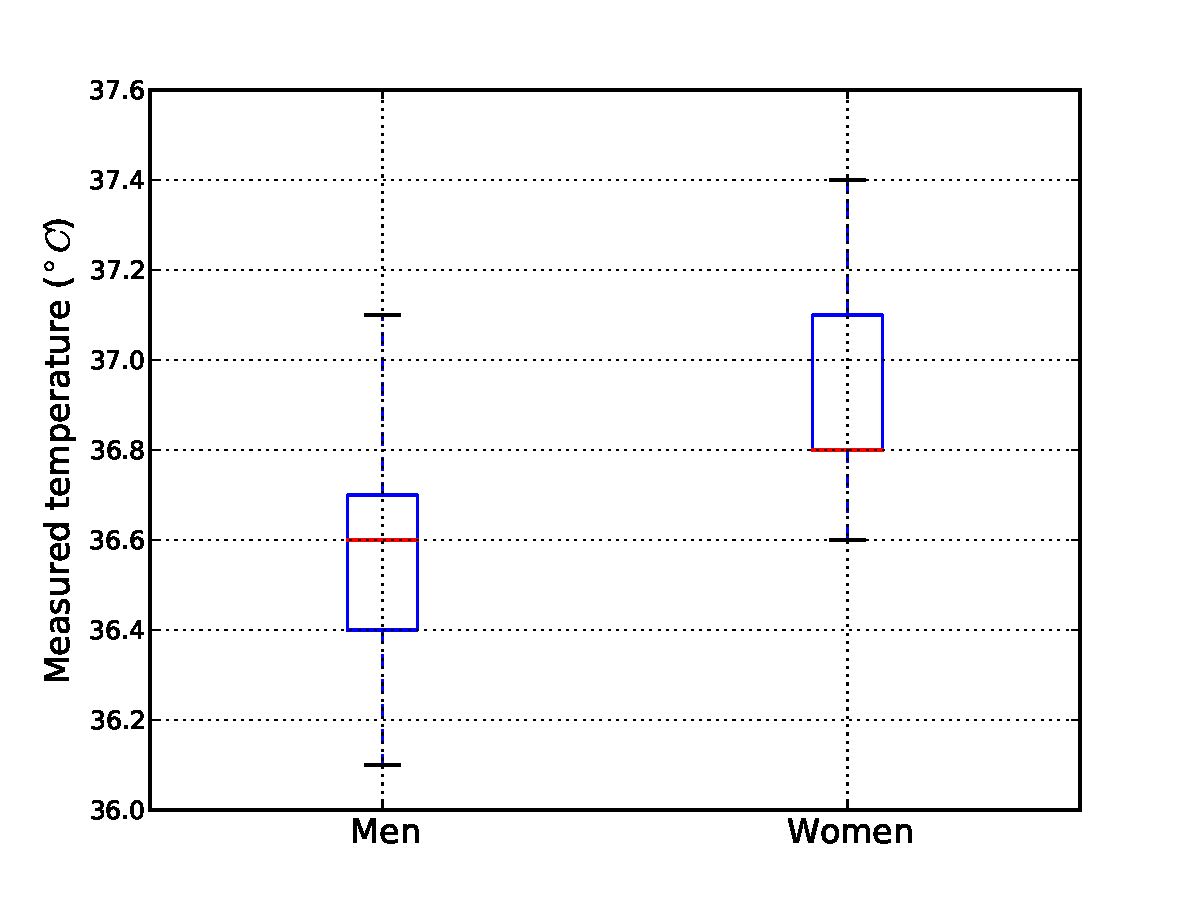
\includegraphics[width=\textwidth]{boxplot.pdf}
\caption{Boxplots of the observations given in table \ref{table:temp}. \label{fig:boxplot}}
\end{figure}

\clearpage

\subsection*{b) Constucting normal probability plots}
We will now check if we can make an assumption about the observations being drawn from a normal distribution by constructing probability plots for our data sets, see figure \ref{fig:probplot}. 

If our observations did follow a normal distribution, we would expect the values shown to lie close to a straight line. In our case, we see that the values does not seem to overwhelmingly support this statement. At the same time, we have to remember that we have very small sample sizes, see the following quote:

\begin{quote} There is typically greater variation in the appearance of the probability plot for sample sizes smaller than 30, and only for much larger sample sizes does a linear pattern generally predominate. When a plot is based on a small sample size, only a very substantial departure from linearity should be taken as conclusive evidence of nonnormality.

\em Devore and Berk, p.\ 212.
\end{quote}

As both of our sample sizes is substantially less than 30, we should not be surprised by the lack of linearity in our probability plots, and they might very well follow a normal distribution, thought it is hard to say anything conclusive with such small sample sizes.

\begin{figure}[htpb]
\centering
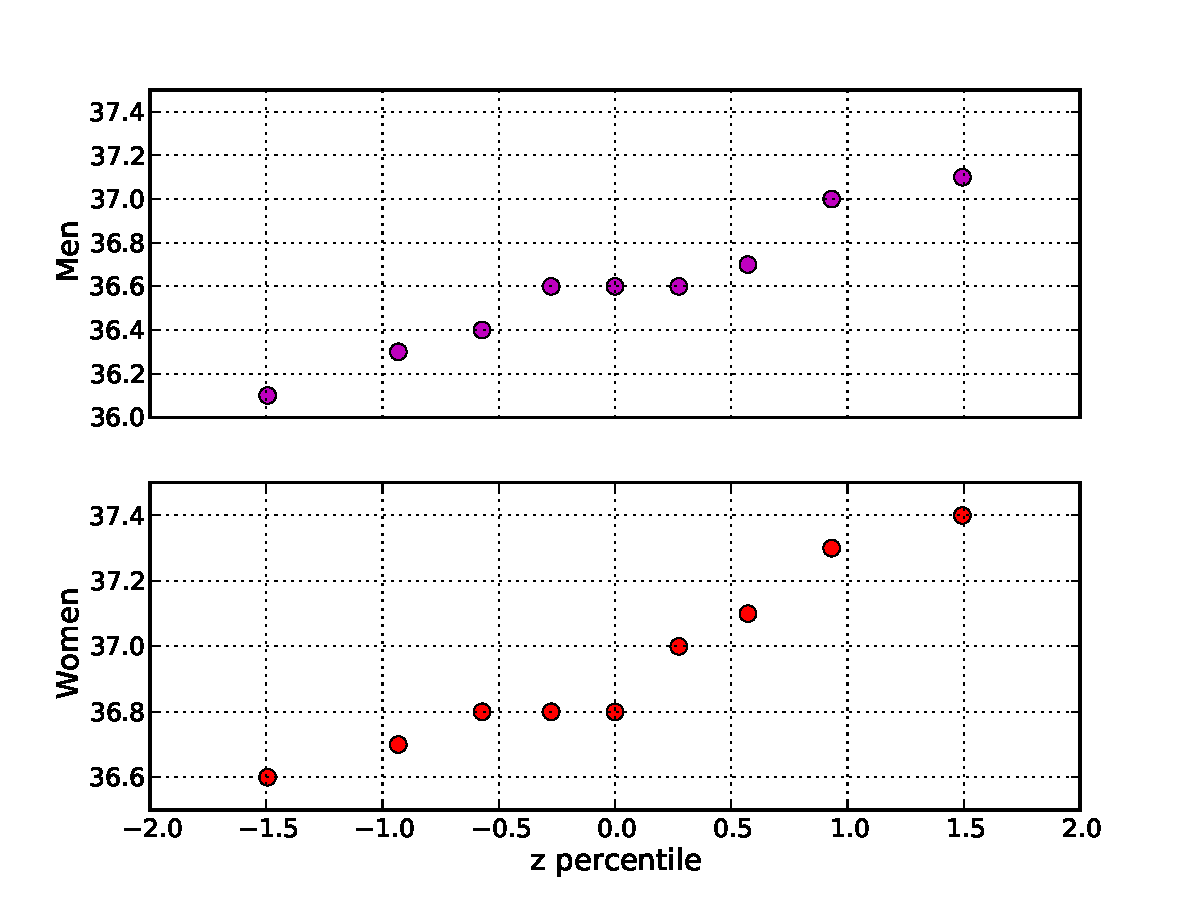
\includegraphics[width=\textwidth]{probabilityplot.pdf}
\caption{Normal probability plot for the observations given in table \ref{table:temp}. \label{fig:probplot}}
\end{figure}

\clearpage

Despite the inconclusiveness of our normal probability plots, we will for the rest of exercise 1 assume that both data sets follow a normal distribution:
$$X \sim \mbox{norm}(\mu_x, \sigma_x),\qquad Y \sim \mbox{norm}(\mu_y, \sigma_y).$$
We will also assume that $X$ and $Y$ are independent. From now on, we will take $X$ to be the measured body temperature of a healthy woman, and $Y$ to be the measurement from a man.

\subsection*{c) Pooled $t$ test and confidence interval}
We will now perform a pooled two-sample $t$ test on our data sets, and test wether there is a difference in expected body temperature for men and women. We will construct a 95\% confidence interval for the difference.

We are interested in the difference in expected body temperature for men and women, an unbiased estimator for this value is
$$\hat{\theta} = \overline{X} - \overline{Y}.$$
The variance of the estimator becomes
$$V(\hat{\theta}) = V(\overline{X}) + V(\overline{Y}) = \frac{\sigma_1^2}{n} + \frac{\sigma_2^2}{m} = \sigma_{\hat{\theta}}^2.$$
We then construct a test statistic 
$$\frac{\hat{\theta} - \Delta_0}{\sigma_{\hat{\theta}}} = \frac{\overline{X} - \overline{Y} - (\mu_1 - \mu_2)}{\sqrt{\frac{\sigma_1}{n} + \frac{\sigma_2}{m}}},$$
where $\Delta_0$ is the null value for $\mu_1 - \mu_2$. As the variances $\sigma_1^2$ and $\sigma_2^2$ are unknown to us, we will have to estimate these using the sample variances. 

To construct a pooled test procedure, we must first make the assumption that the variance of the two normal distributions is equal:
$$\sigma_x^2 = \sigma_y^2 = \sigma^2.$$
Now, we still don't know what $\sigma^2$ is, we just know assume that it is equal for the two distributions. To estimate it, we use the pooled estimator
$$S_p^2 = \frac{m-1}{m+n-2}S_1^2 + \frac{n-1}{m+n-2}S_2^2,$$
where $m$ and $n$ are the sample sizes of the data set and $S_1^2$ and $S_2$ are the sample variances. As we have an equal number of samples in both data sets, the pooled estimator is simply the arithmetic average. Calculating the sample variances from
$$S = \frac{1}{n-1}\sum_{i=1}^n (y_i - \overline{y})^2,$$
yields
$$S_x^2 = 0.0753, \qquad S_y^2 = 0.1,$$
and so the pooled estimator is
$$S_p^2 = \frac{S_x^2 + S_y^2}{2} = 0.08765.$$
If we replace both $\sigma_1^2$ and $\sigma_2^2$ with the pooled estimator in the test statistic, we have
$$t = \frac{\overline{X} - \overline{Y} - \Delta_0}{\sqrt{S_p^2\bigg(\frac{1}{m} + \frac{1}{n}\bigg)}}.$$
Altough we will not show it, this test statistic has a $t$ distribution, see \emph{Devore and Berk} p.\ 497 for a proof of this. Our null hypothesis is now
$$H_0: \mu_1 - \mu_2 = \Delta_0,$$
and the alternative hypothesises are
\begin{table}[htpb]
\begin{tabular}{l | l}
Alternative hypothesis & Rejection region for approximate level $\alpha$ test \\ \hline
$H_a: \quad \mu_1 -\mu_2 > \Delta_0$ & $t\geq t_{\alpha, \nu}$ \\ \hline
$H_a: \quad \mu_1 -\mu_2 < \Delta_0$ & $t\leq -t_{\alpha, \nu}$ \\ \hline
$H_a: \quad \mu_1 -\mu_2 \neq \Delta_0$ & $t\geq t_{\alpha/2, \nu}$ or $t\leq -t_{\alpha/2, \nu}$ \\ \hline
\end{tabular}
\caption{Alternate hypothesises and rejection regions for a $t$ test. Table gotten from }
\end{table}

Before we can conduct any $t$ test on our data set, we must find the value of $\nu$, it can be estimated directly from the data by\footnote{See \emph{Devore and Berk} p.\ 487.}
$$\nu = \left\lfloor\frac{\bigg(\frac{s_1^2}{m} + \frac{s_2^2}{n}\bigg)^2}{\frac{(s_1^2/m)^2}{m-1} + \frac{(s_2/n)^2}{n-1}}\right\rfloor.$$
For the pooled $t$ test, we insert the pooled estimator for both $s_1^2$ and $s_2^2$ and find that
$$\nu_p = 16.$$

Testing the null hypothesis $\Delta_0 = 0$ with a level $\alpha = P(\mbox{type I error}) = 0.05$, yields
$$t = 2.468 \geq t_{0.025, 16} = 2.12.$$
So we see that the null hypothesis of $\Delta_0 = 0$ is rejected at this level. The $p$-value becomes
$$p = 2(.012) = 0.024.$$
A 95\% confidence interval for the difference $\mu_1 - \mu_2$ is given by
$$\overline{x} - \overline{y} \pm t_{0.025, 16}\sqrt{S_p^2\bigg(\frac{1}{n}+\frac{1}{m}\bigg)}.$$
Which becomes
$$\mu_1 - \mu_2 \in (0.048, 0.640). $$

\subsection*{d) Unpooled two-sample $t$ test and confidence interval}

We will now perform another $t$ test, but this time we will make no assumption about the real variances being similar. We then use the test statistic
$$t = \frac{\overline{x} - \overline{y}- \Delta_0}{\sqrt{\frac{S_1^2}{n} + \frac{S_2^2}{m}}}.$$
The test statistic is still $t$ distributed, but we must calculate $\nu$ anew
$$\nu = \left\lfloor\frac{\bigg(\frac{s_1^2}{m} + \frac{s_2^2}{n}\bigg)^2}{\frac{(s_1^2/m)^2}{m-1} + \frac{(s_2/n)^2}{n-1}}\right\rfloor = 15.$$
Again we test the null hypothesis $\Delta_0 = 0$, and find
$$t = 2.468 \geq t_{0.025, 15} = 2.131.$$
So we see that the null hypothesis is still rejected at the level $\alpha = 0.05$. The $p$-value is now
$$p = 2(0.012) = 0.024,$$
which is identical to the $p$ value in the pooled test.

The 95\% confidence interval is now given by
$$\overline{x} - \overline{y} \pm t_{0.025, 15}\sqrt{\frac{S_1^2}{n}+\frac{S_2^2}{m}},$$
which gives
$$\mu_1 - \mu_2 \in (0.047, 0.642).$$

\subsubsection*{Verifying using R}

To verify that we have constructed the correct tests and done the right calculations, we run our data sets through the $R$-procedure \verb+t.test()+. The code is very simple
\begin{lstlisting}
> x = c(36.6, 36.7, 36.8, 36.8, 36.8, 37.0, 37.1, 37.3, 37.4)
> y = c(36.1, 36.3, 36.4, 36.6, 36.6, 36.6, 36.7, 37.0, 37.1)
> t.test(x,y)
> t.test(x,y, var.equal=T)
\end{lstlisting}

The command \verb+t.test(x,y)+ runs the (unpooled) two-sample $t$ test for the null value $\Delta_0 = 0$, it gives the following output

\begin{lstlisting}
	Welch Two Sample t-test

data:  x and y
t = 2.4682, df = 15.688, p-value = 0.02549
alternative hypothesis: true difference in means is not equal to 0
95 percent confidence interval:
 0.04812421 0.64076468
sample estimates:
mean of x mean of y 
 36.94444  36.60000 
\end{lstlisting}

The command \verb+t.test(x,y, var.equal=T)+ runs the pooled $t$ test, with the following output

\begin{lstlisting}
	Two Sample t-test

data:  x and y
t = 2.4682, df = 16, p-value = 0.02524
alternative hypothesis: true difference in means is not equal to 0
95 percent confidence interval:
 0.04860326 0.64028563
sample estimates:
mean of x mean of y 
 36.94444  36.60000 
\end{lstlisting}

We see that our results come very close to those produced by R. I suspect the small differences are a result of the bad $t$-resolution of the table A.8 in \emph{Devore and Berk}.

\subsubsection*{Discussion}

We have seen that for both the pooled and unpooled two sample $t$ tests that the null hypothesis $H_0: \mu_1 - \mu_2$ has been rejected at the level $\alpha = 0.05$, and in both cases found a $p$-value of approximately 0.025. This means that it is highely unlikely that the differences in the measured body temperatures of the men and women sampled is a result caused by chance. We also see from the 95\% confidence intervals constructed for $\mu_1 - \mu_2$ that it is very likely that the healty women of the population have a higher body temperature than the men.

\clearpage

\subsection*{e) Constructing an F-test}

We will now construct an $F$-test to test the hypothesis $H_0: \sigma_1^2 = \sigma_2^2$.

We know that if we have to independent normal distributions, then
$$F = \frac{S_1^2/\sigma_1^2}{S_2^2/\sigma_2^2},$$
will be $F$ distributed with $v_1 = m-1$ and $v_2 = n-1$. Under our hypothesis, we can then construct the test statistic
$$f = s_1^2/s_2^2,$$
which will be $F$-distributed with $\nu_1 = \nu_2 = 8$.

We then have the alternative hypothesis $H_a: \sigma_1^2 \neq \sigma_2^2$ with the rejection region for an $\alpha$-level test:
$$f \geq F_{\alpha/2,\nu_1,\nu_2} \mbox{  or  } f \leq F_{1-\alpha/2,\nu_1,\nu_2}.$$
We now perform the test on our data sets with $\alpha=0.10$, and find
$$f = s_1^2/s_2^2 = 0.753,$$
while
$$F_{0.05, 8, 8} = 3.44, \qquad F_{0.95, 8, 8} = \frac{1}{F_{0.05, 8, 8}} = \frac{1}{3.44} = 0.291.$$
We see that the null hypothesis stands. We could also find a $p$-value for the $F$-test and a 95\% confidence interval for the ratio, but let us simply let R calculate those for us. The command
\begin{lstlisting}
> var.test(x, y)
\end{lstlisting}
gives the output
\begin{lstlisting}
	F test to compare two variances

data:  x and y
F = 0.7528, num df = 8, denom df = 8, p-value = 0.6975
alternative hypothesis: true ratio of variances is not equal to 1
95 percent confidence interval:
 0.1698023 3.3372595
sample estimates:
ratio of variances 
         0.7527778 
\end{lstlisting}
So we see that the 95\% confidence interval is
$$\frac{\sigma_1}{\sigma_2} \in (0.170, 3.34).$$
and that the $p$-value for $H_0$ is $p=0.6975$.

We see that there is little reason to reject the null asumption that the variances are equal.

\subsection*{f) Prediction interval}

We now look at the case where a new measurement is to be taken for each gender. We will be looking at the difference in these measurements $X_{10} - Y_{10}$. We now assume that $X\sim \mbox{norm}(\mu_1, \sigma)$ and $Y\sim \mbox{norm}(\mu_1, \sigma)$.

A reasonable prediction for $X_{10} - Y_{10}$ is $\overline{X} - \overline{Y}$, this is apparent from the expectation values
$$E(X_{10} - Y_{10}) = E(X_{10}) - E(Y_{10}) = \mu_1 - \mu_2.$$
$$E(\overline{X} - \overline{Y}) = E(\overline{X}) - E(\overline{Y}) = \mu_1 - \mu_2.$$
$$E(X_{10} - Y_{10}) = E(\overline{X} - \overline{Y}).$$

We can also define a stochastic variable
$$P = X_{10} - Y_{10} - (\overline{X} - \overline{Y}),$$
which will be normally distributed as it is a linear combination of normally distributed variables. The expectation value is simply
$$E(P) = E(X_{10} - Y_{10}) - E(\overline{X} - \overline{Y}) = 0.$$
And the variance becomes
$$V(P) = V(X_{10}) + V(Y_{10}) + V(\overline{X}) + V(\overline{Y}) = \frac{20}{9}\sigma^2.$$
So we see that
$$P \sim \mbox{norm}(0, 20\sigma^2/9).$$
This means we can construct a standard normal variable
$$Z = \frac{9P}{20\sigma^2}.$$
And a 95\% confidence interval for $X_{10} - Y_{10}$ is then given by
$$\overline{X}-\overline{Y} \pm z_{0.025}\cdot \frac{20\sigma^2}{9}.$$
As $\sigma^2$ is not known, we estimate it using the pooled estimator (as we are assuming $X$ and $Y$ have the same variance), giving the prediction interval
$$X_{10} - Y_{10} \in (-0.037, 0.726).$$

We can compare this to the confidence interval found earlier:
$$\mu_1 - \mu_2 \in (0.047, 0.642).$$

A confidence interval is a measure of how well we have determined a parameter of a population, in this case the difference between the means. This means that if we had a lot of data on the population, the confidence interval would be very narrow, as the true value of the parameter is well known. The prediction interval however, must also account for the variance of the data itself. So even if we had a lot of data on a population, the prediction interval might still be quite wide, if the population has a high variance. To summarize: the prediction interval has to account for both our lacking knowledge of the true parameter value, as well as the variance in the data itself. This effectively means that a prediction interval is always wider than a confidence interval, which we see is the case for our intervals aswell.


\clearpage

\subsection*{Exercise 2}

We have the following data

\begin{table}[h]
\centering
\begin{tabular}{l | c | c | c | c}
& n	& $\overline{x}$ & $s$	& $s/\sqrt{n}$ \\ \hline
Twin A 	& 31 & 93.32 & 15.41 & 2.77 \\ \hline
Twin B 	& 31 & 96.58 & 13.84 & 2.49 \\ \hline
Difference & 31 & -3.26 & 8.81 & 1.58 
\end{tabular}
\caption{Data from twin study.}
\end{table}

\subsection*{a)}
A paired $t$ test is best in this case, due to the nature of the twin pairs. As every twin has been selected for the study as a pair, no claim can be made to the measurements of twin A and twin B being independent, and so a two-sample $t$ test is not possible. We can however assume that the selection of every pair of twins is independent, in fact, we must make this assumption to perform a paired $t$ test on the data. We must also assume that the differences are normally distributed
$$D \sim \mbox{norm}(\mu_D, \sigma_D^2).$$

\subsection*{b)}
The expectation value of $D$ in each case is $E(D) = \mu_D$. We formulate a null hypothesis $H_0: \mu_D = 0$. Our test statistic is then
$$t = \frac{\overline{d} - \Delta_0}{s_D/\sqrt{n}},$$
which is $t$ distributed with $\nu = n-1 = 30$ degrees of freedom. The alternative hypothesis is $H_a: \mu_D \neq \Delta_0$, with a rejection region for a level $\alpha$ test:
$$t \geq t_{\alpha/2, n-1} \mbox{  or  } t\leq-t_{\alpha/2, n-1}.$$
For our data, the numerical value of the test statistic is
$$t = -3.26/1.58 = -2.06.$$
The $p$-value becomes $2(0.022) = 0.044$.

The low $p$-value indicates that the null hypothesis would be discarded in a $\alpha=0.05$ test. Thus the alternative hypothesis that there is in fact a real difference between the expected value of IQ of twin A and B, i.e.\ $\mu_D \neq 0$, seems to be correct.

\subsection*{c)}
We will now construct a 95\% confidence interval for $\mu_D$. Our test statistic
$$t = \frac{\overline{d} - \mu_D}{s_D/\sqrt{n}},$$
was $t$-distributed with $n-1=30$ degrees of freedom. A 95\% confidence interval for $\mu_D$ is then
$$\overline{d} \pm t_{0.025, 30}\cdot s_D/\sqrt{n},$$
and so we find that to 95\% confidence
$$\mu_D \in (-6.49, -0.03).$$

The fact that the whole 95\% confidence interval is negative indicates the fact that the true average of the difference between Twin A and Twin B, $\mu_D$, is negative. This again indicated that the true mean of the IQ of Twin B, $\mu_B$ is larger than that of Twin A, $\mu_A$.

\section*{Exercise 3}

A survey is conducted and answers gathered from 3000 fathers, and 3000 mothers. Of these, 486 men and 441 women answered in the positive, and the rest in the negative. We want to examine if the difference in answers is significant, or within a reasonable variation.

Let us name the true proportions of the population of fathers and mothers who would answer positive to be $p_1$ and $p_2$ respectively. We will assume that the answers given by the fathers and mothers to be independent. We also assume that the population size of both fathers and mothers to be much larger than the number surveyed. The number of fathers and mothers who anser positively in the survey will then follow a near binomic distribution:
$$X \sim \mbox{Bin}(m, p_1), \qquad Y \sim \mbox{Bin}(n, p_2).$$

We are interested in studying the difference in the true proportions: $p_1 -p_2$. An unbiased estimator for this difference is
$$\hat{\theta} = \hat{p}_1 - \hat{p}_2 = \frac{X}{m} - \frac{Y}{n},$$
the variance becomes
$$V(\hat{\theta}) = V(\hat{p}_1) + V(\hat{p}_2) = \frac{p_1q_1}{m} + \frac{p_2q_2}{n}.$$
As we have very large sample sizes ($n=m=3000$), we will now construct a large-sample test procedure. The binomic distribution of $X$ and $Y$ can be approximated by a normal distribution for large sample sizes, so we can construct an approximately standard normal distribution
$$Z = \frac{\hat{p}_1 - \hat{p}_2 - (p_1 - p_2)}{\sqrt{\frac{p_1q_1}{m} + \frac{p_2q_2}{n}}}.$$
And from this we can create our test statistic by replacing $p_1 - p_2$ by the null value $\Delta_0$. In our case, we formulate the null hypothesis: 
$$H_0: p_1 - p_2 = \Delta_0 = 0,$$
meaning we assume $p_1 = p_2 = p$. In that case, the test statistic simplifies to
$$z = \frac{\hat{p}_1 - \hat{p}_2}{\sqrt{pq\bigg(\frac{1}{m} + \frac{1}{n}}\bigg)},$$
but in this case, $p$ is of course unknown, so we use a weighted average of the estimators $\hat{p}_1$ and $\hat{p}_2$:
$$\hat{p} = \frac{X + Y}{m + n} = \frac{m}{m+n}\hat{p}_1 + \frac{n}{m+n}\hat{p}_2.$$
As $m=n$ in this case, the average simplifies to the arithmetic mean and the test statistic takes the form
$$z = \frac{\hat{p}_1 - \hat{p}_2}{\sqrt{\frac{1}{n}(\hat{p}_1 + \hat{p}_2)(1 - \frac{\hat{p}_1 + \hat{p}_2}{2})}}.$$

The alternative hypothesis is
$$H_a: p_1 - p_2 \neq 0.$$
As the test statistic is approximately standard normal, the rejection region is simply
$$z \geq z_{\alpha/2} \mbox{  or  } z \leq -z_{\alpha/2}.$$

We calculate the $z$-value for our data and find the corresponding $p$-value
$$z = 1.60.$$
$$p\mbox{-value} = 2[1-\Phi(z)] = 2[1-\Phi(1.60)] = 0.11.$$

We see that the null hypothesis---that there is no difference in the real proportions in the population of fathers and mothers---is not rejected at a $\alpha=0.05$ level test. We also see that the $p$-value is not too low. The conclusion is thus that the results of the survey are not significant enough to claim that there is a real difference between the populations.

\clearpage

\section*{Exercise 4}

Table \ref{table:snow} shows measurements of both the amount of snow in winter and the water-level in spring over 18 years. We let the amount of snow be the predictor variable, 
$x$, and the water-level be the response variable $y$. Figure \ref{fig:scatter} shows the data in a scatter plot.

\vspace{1cm}

\begin{table}[h]
\centering
\begin{tabular}{l | c | c | c | c | c | c | c | c | c }
Snow  & 10.5 & 16.7 & 18.2 & 17.0 & 16.3 & 10.5 & 23.1 & 12.4 & 24.9 \\ \hline
      & 22.8 & 14.1 & 12.9 & 8.80 & 17.4 & 14.9 & 10.5 & 10.5 & 16.1 \\ \hline
Water & 23.1 & 32.8 & 31.8 & 32.0 & 30.4 & 24.0 & 39.5 & 24.2 & 52.5 \\ \hline
      & 37.9 & 30.5 & 25.1 & 12.4 & 35.1 & 31.5 & 21.1 & 27.6 & 27.6 
\end{tabular}
\caption{Measurements of snow and water levels. \label{table:snow}}
\end{table}

\begin{figure}[htpb]
\centering
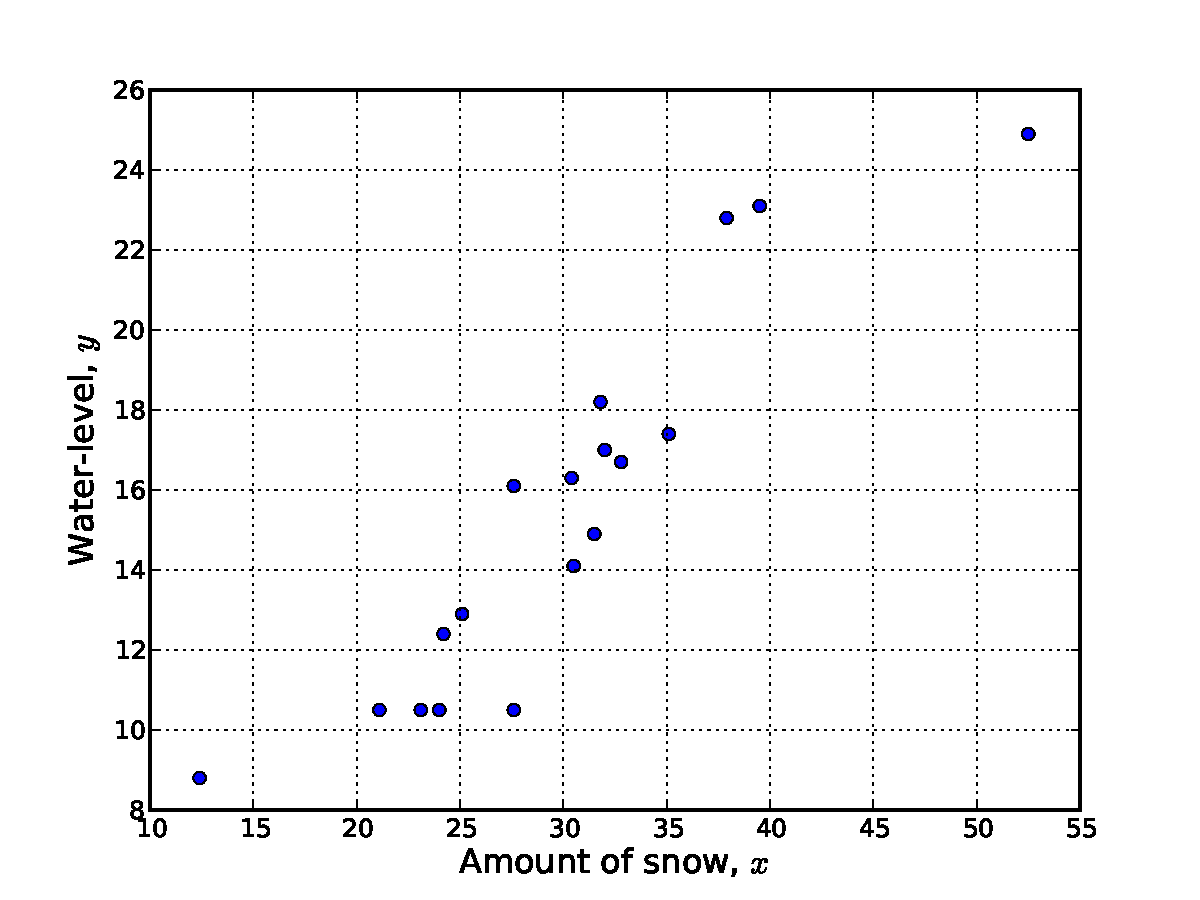
\includegraphics[width=\textwidth]{scatter.pdf}
\caption{Scatter plot of data given in table \ref{table:snow}. \label{fig:scatter}}
\end{figure}

\clearpage

\subsection*{a) A linear regression model}

From the scatter plot, a simple linear regression model seems appropriate. We then define the stochastic variable
$$Y = \beta_0 + \beta_1x + \varepsilon, \qquad \varepsilon \sim \mbox{norm}(0,\sigma^2).$$
To fit $Y$ to our data, we must estimate the parameters $\beta_0$, $\beta_1$ and $\sigma^2$. This can be done using the principle of least squares.

For simplicity, we feed the data into R, and use the method \verb+lm()+ to estimate $\beta_0$ and $\beta_1$. 
\begin{lstlisting}
> lm(y ~ x)
\end{lstlisting}
which gives the following output
\begin{lstlisting}
Call:
lm.r = lm(signal ~ conc)
lm(formula = y ~ x)

Coefficients:
(Intercept)            x  
     0.2800       0.5056  
\end{lstlisting}
And so the estimated deterministic linear relationship between $x$ and $y$ is
$$y = 0.28 + 0.5056x.$$
We plot this line into the scatter plot shown on the last page, the resulting plot is shown in figure \ref{fig:reg}. From the figure, we see that the calculated coefficients seem reasonable.

\begin{figure}[htpb]
\centering
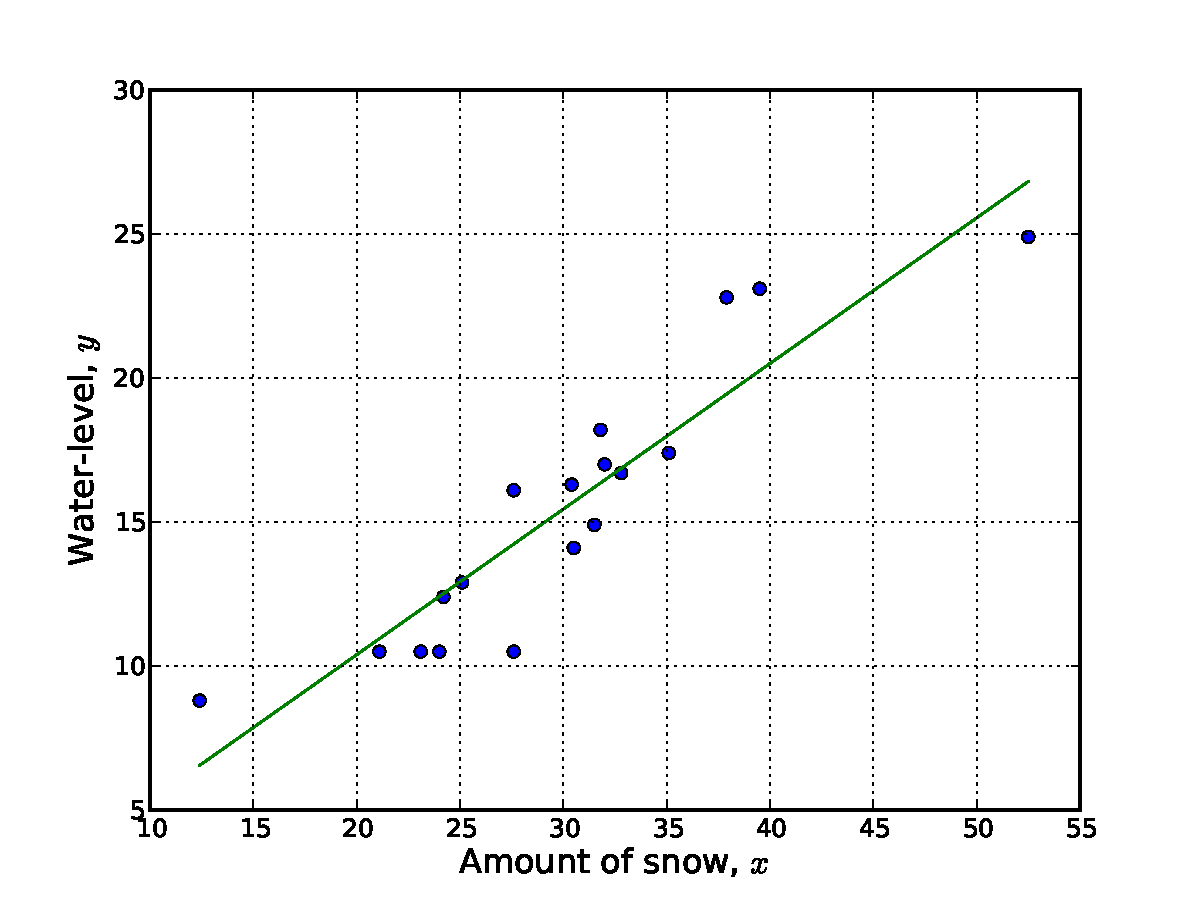
\includegraphics[width=0.9\textwidth]{fittedreg.pdf}
\caption{Observed data and fitted linear regression line. \label{fig:reg}}
\end{figure}

\clearpage

\subsection*{b) Checking normalcy of the residuals}
We now calculate the residuals, which is defined as the vertical deviations from the deterministic linear relationship, $y_i - \hat{y}_i$. We plot the residuals agains the predictor value $x$, see figur \ref{fig:residuals}. We also make a probability plot to examine the normalcy of the residuals, this is done similar to exercise 1b, see figure \ref{fig:probplot2}. We see that the residuals in the probability plot seem to lie on a straight line, indicating that they are following a normal distribution. This means that our linear regression model seems reasonable.

\begin{figure}[htpb]
\centering
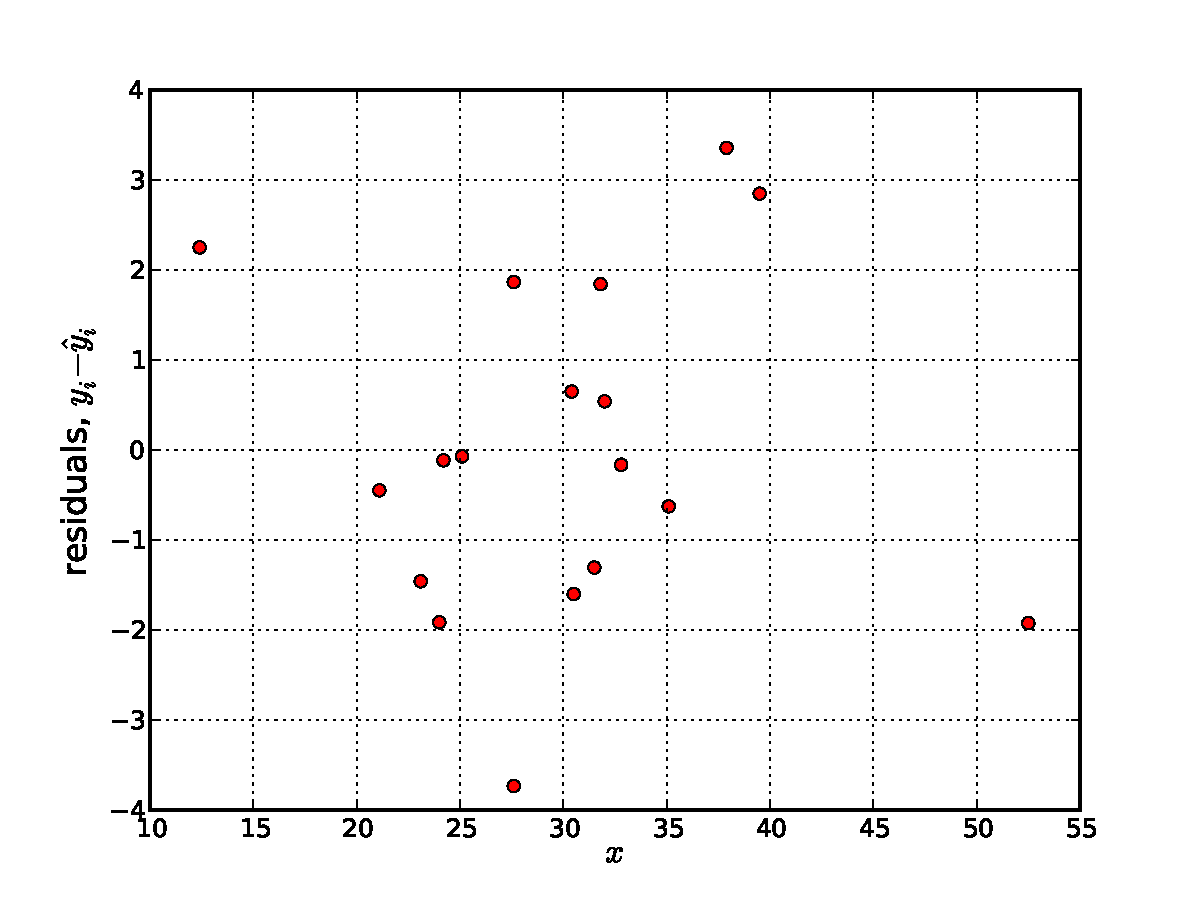
\includegraphics[width=0.8\textwidth]{residuals.pdf}
\caption{Residuals plotted against the predictor values. \label{fig:residuals}}
\end{figure}

\begin{figure}[htpb]
\centering
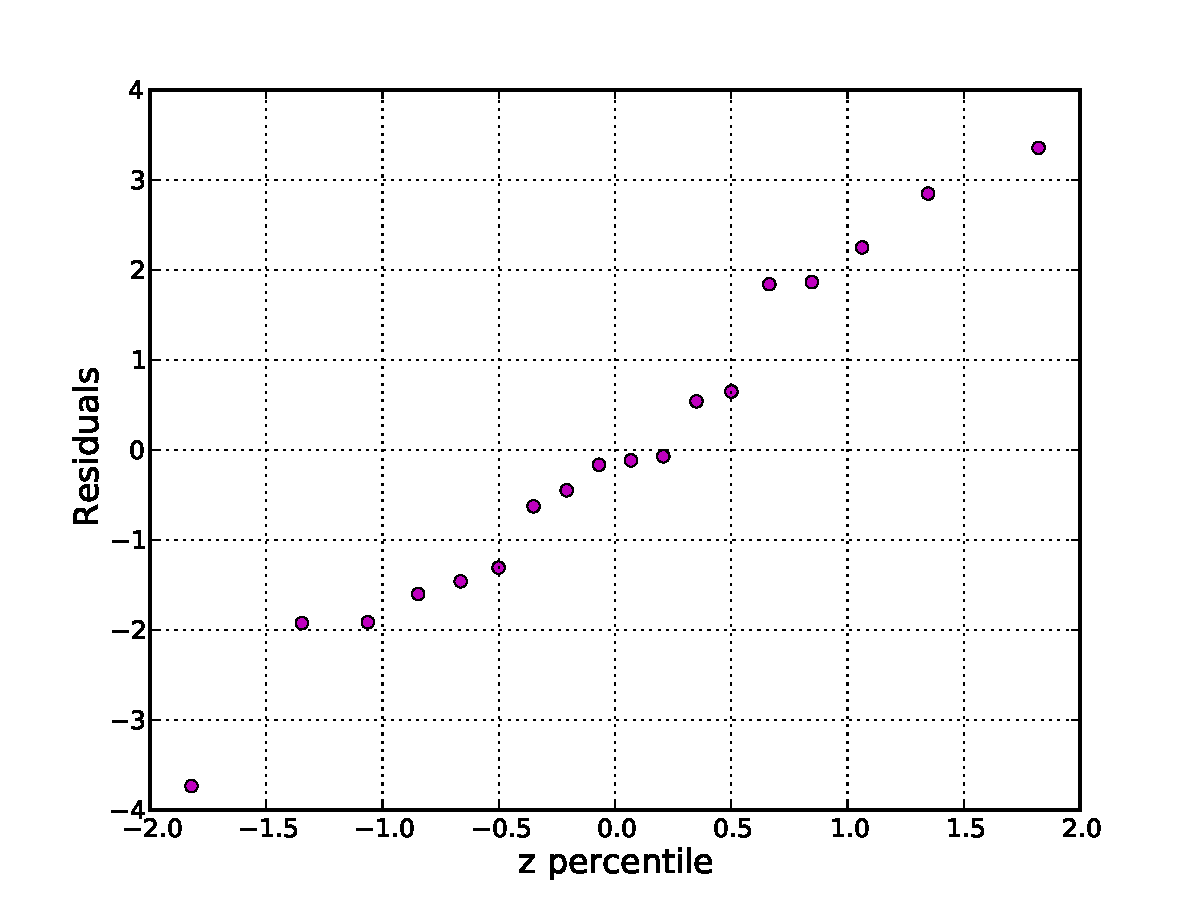
\includegraphics[width=0.8\textwidth]{probabilityplot2.pdf}
\caption{Probability plot of residuals. \label{fig:probplot2}}
\end{figure}


\end{document}

